\documentclass[11pt,a4paper]{article}
\usepackage[margin=2.2cm]{geometry}
\usepackage{amsmath,amssymb,bm}
\usepackage{booktabs,longtable,array}
\usepackage{graphicx}
\usepackage{xcolor}
\usepackage{tikz}
\usetikzlibrary{arrows.meta,positioning,fit,calc,backgrounds,shapes.geometric}
\usepackage[colorlinks=true,linkcolor=blue!50!black,urlcolor=blue!50!black]{hyperref}
\usepackage{caption}
\usepackage[htt]{hyphenat}
\usepackage{needspace}
\usepackage[section]{placeins}
\sloppy

\newcommand{\code}[1]{\texttt{\small #1}}
\newcommand{\pass}{\textcolor{green!45!black}{\textbf{PASS}}}
\newcommand{\fail}{\textcolor{red!70!black}{\textbf{FAIL}}}
\newcommand{\Sc}{\mathcal S}

\title{Entropy Stable Neural ROM (1D periodic FV)\\[2pt]
\large Method, code structure and unit test report}
\author{Atakan Aygun -- AMiP \quad (code: \code{ES-ROM/ROM/})}
\date{\today}

\begin{document}
\maketitle

\begin{abstract}
This report documents the PyTorch implementation of the entropy stable neural reduced order model of \code{es\_nn\_rom\_fv1d\_plan.md}. The network is the reduced model, $M\dot a=(J_\theta(a)-R_\theta(a))\,v_N(a)$, with skew $J_\theta$ and positive semi-definite $R_\theta$. The entropy variables $v_N$ come from the physics. Sections~\ref{sec:fom}--\ref{sec:coupling} describe how the FOM data are obtained, the reduced space, the network, how entropy stability is built in, and how the pieces are coupled. Section~\ref{sec:tests} reports the unit tests. Each test file was run separately, each test individually, with the measured value of every invariant. \textbf{All 33 tests pass} (one test reference was corrected, see Sec.~\ref{sec:t-physics}). The total test time is about 20\,s. Section~\ref{sec:results} compares trained models with the FOM for Burgers. Keeping Chan's ES-ROM exact and learning only an entropy-admissible eddy viscosity (Sec.~\ref{sec:closure}) halves the ES-ROM's end-time error at $r=6$.
\end{abstract}

\tableofcontents

%======================================================================
\section{Obtaining the FOM data}\label{sec:fom}
%======================================================================

\subsection{Full order model}
The FOM is Chan's entropy stable finite volume scheme (Chan 2020, Sec.~2) on a uniform periodic grid of $K$ cells on $[-1,1]$, with $\Delta x = 2/K$:
\begin{equation}\label{eq:fom}
\Delta x\,\frac{du}{dt} + 2(Q\circ F)\mathbf 1 + \epsilon K_{\rm lap}u = 0,\qquad F_{ij}=f_S(u_i,u_j).
\end{equation}
\begin{itemize}
\item $Q$ is the periodic central difference ($+\tfrac12$ superdiagonal, $-\tfrac12$ subdiagonal). Since $Q$ is tridiagonal, $\big(2(Q\circ F)\mathbf 1\big)_i = f_S(u_i,u_{i+1})-f_S(u_{i-1},u_i)$. This is a difference of edge fluxes, so the cost is $O(K)$ and $F$ is never formed (\code{utils/fom.py:62}, \code{FOM1D.conv}).
\item $K_{\rm lap} = \tfrac{1}{\Delta x}\,\mathrm{tridiag}(-1,2,-1)=\Delta x D^TD$, the same scaling as \code{FOM/esrom/operators.py} (\code{FOM1D.visc}, line 67).
\item $f_S$ is entropy conservative: Tadmor's condition $(v_L-v_R)^Tf_S=\psi_L-\psi_R$ holds. Therefore $v^T 2(Q\circ F)\mathbf 1 = 0$, and the only entropy change is viscous:
\begin{equation}\label{eq:fomdiss}
\frac{d\Sc}{dt} = \Delta x\,v^T\dot u = -\epsilon\, v^TK_{\rm lap}u \le 0,\qquad \Sc(u)=\Delta x\textstyle\sum_i S(u_i).
\end{equation}
\end{itemize}

\paragraph{Physics} (\code{utils/physics.py}, PyTorch float64, states stored as $(\dots,n_{var},K)$):
\begin{itemize}
\item \textbf{Burgers}: $S=u^2/2$, $v=u$, $f_S=(u_L^2+u_Lu_R+u_R^2)/6$, $\psi=u^3/6$. The entropy projection is trivial here, so Burgers only tests the plumbing.
\item \textbf{Euler}: $S=-\rho s$ with $s=\log(p/\rho^\gamma)$ and $\gamma=1.4$. The entropy variables $v(u)$ and their inverse $u(v)$ are coded in closed form. The flux is Chandrashekar's EC flux. The logarithmic mean uses the Ismail--Roe series for $|f|^2<10^{-4}$ and a ``double \code{where}'', so that gradients stay finite.
\end{itemize}

\paragraph{Time integration.} Carpenter--Kennedy 5-stage, 4th-order low-storage RK (\code{utils/fom.py:27,36}).

\subsection{Snapshot generation}
\code{generate\_snapshots} (\code{utils/fom.py:100}) integrates \eqref{eq:fom} to $T_{\rm final}$ and stores every \code{SAVE\_EVERY} steps:
\begin{center}
\begin{tabular}{p{2.9cm}p{4.0cm}p{8.2cm}}
\toprule
Stored array & Meaning & Used for\\\midrule
$U_k$ & state $u(t_k)$, shape $(N_t,n_{var},K)$ & basis, data inputs $a_k=V^TU_k$, error reference\\
$\dot U_k$ & exact derivative $\mathrm{rhs}_{\rm FOM}(U_k)$ & data targets $\dot a_k=V^T\dot U_k$ (no finite differences)\\
$D_k$ & FOM dissipation $\epsilon v^TK_{\rm lap}u=-d\Sc/dt$ & entropy-rate target\\
$\Sc_k$ & FOM entropy & post-processing\\
\bottomrule
\end{tabular}
\end{center}
\noindent\code{load\_problem} (\code{esnn\_model.py:62}) runs this once per case. It builds the POD basis from the training-window snapshots ($t\le T_{\rm train}$) and caches everything, including $V$, in \code{outputs/<case>/fom.npz}. Training and post-processing therefore always use the same $V$. The cache is regenerated if any setting in Table~\ref{tab:cases} changes.

\begin{table}[h]\centering
\caption{Cases in \code{esnn\_config.py} (\code{ESNN\_QUICK=1} values in parentheses).}\label{tab:cases}
\begin{tabular}{lcc}
\toprule
& Burgers (plumbing) & Euler (target)\\\midrule
initial condition & $u_0=-\sin\pi x$ & $\rho=2+\tfrac12 g$, $u=\tfrac1{10}g$, $p=\rho^\gamma$\\
 & & $g=e^{-100(x-0.5)^2}$\\
$K$ & 1000 (200) & 2500 (500)\\
$\epsilon$ & $2\times10^{-3}$ & $2\times10^{-4}$\\
$\Delta t$ & $5\times10^{-4}$ ($2.5\times10^{-3}$) & $2.5\times10^{-4}$ ($1.25\times10^{-3}$)\\
$T_{\rm train}$ / $T_{\rm final}$ & 0.75 / 1.5 & 0.7 / 2.0\\
saved every & 5 steps & 10 steps\\
modes $r$ per variable; $n=n_{var}r$ & 16, $n=16$ & 16, $n=48$\\
\bottomrule
\end{tabular}
\end{table}

Figure~\ref{fig:fom} shows the cached data from your runs: Burgers at $K=1000$, and the quick Euler case at $K=500$. The full $K=2500$ Euler data have not been generated yet.
\begin{itemize}
\item The FOM entropy decreases monotonically in both cases, as \eqref{eq:fomdiss} requires.
\item The Euler density develops small oscillations behind the steepening fronts for $t\gtrsim0.8$. This is expected for an entropy conservative flux with this little viscosity on the coarse quick grid. It is the data, not a code error, and it makes the extrapolation window ($t>0.7$) the hard part of the problem.
\item The vertical line in the singular value plots is at $r=16$.
\end{itemize}

\begin{figure}[h]\centering
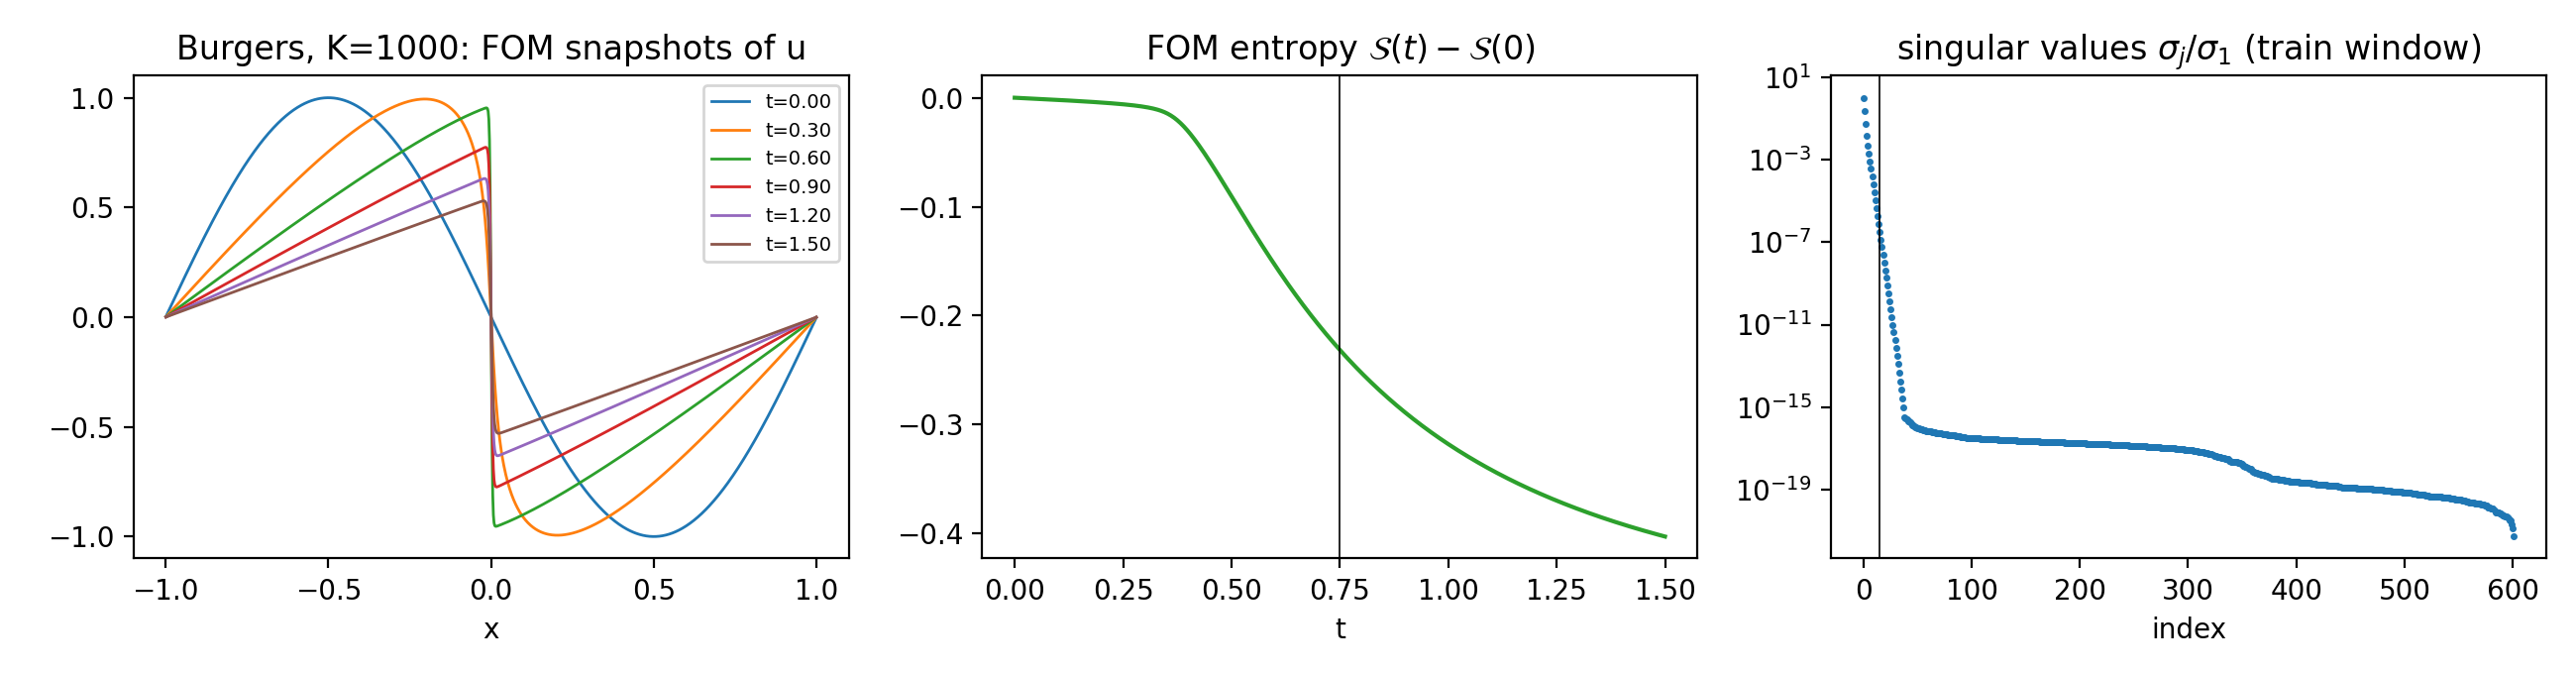
\includegraphics[width=\textwidth]{figs/fom_burgers.png}\\[2pt]
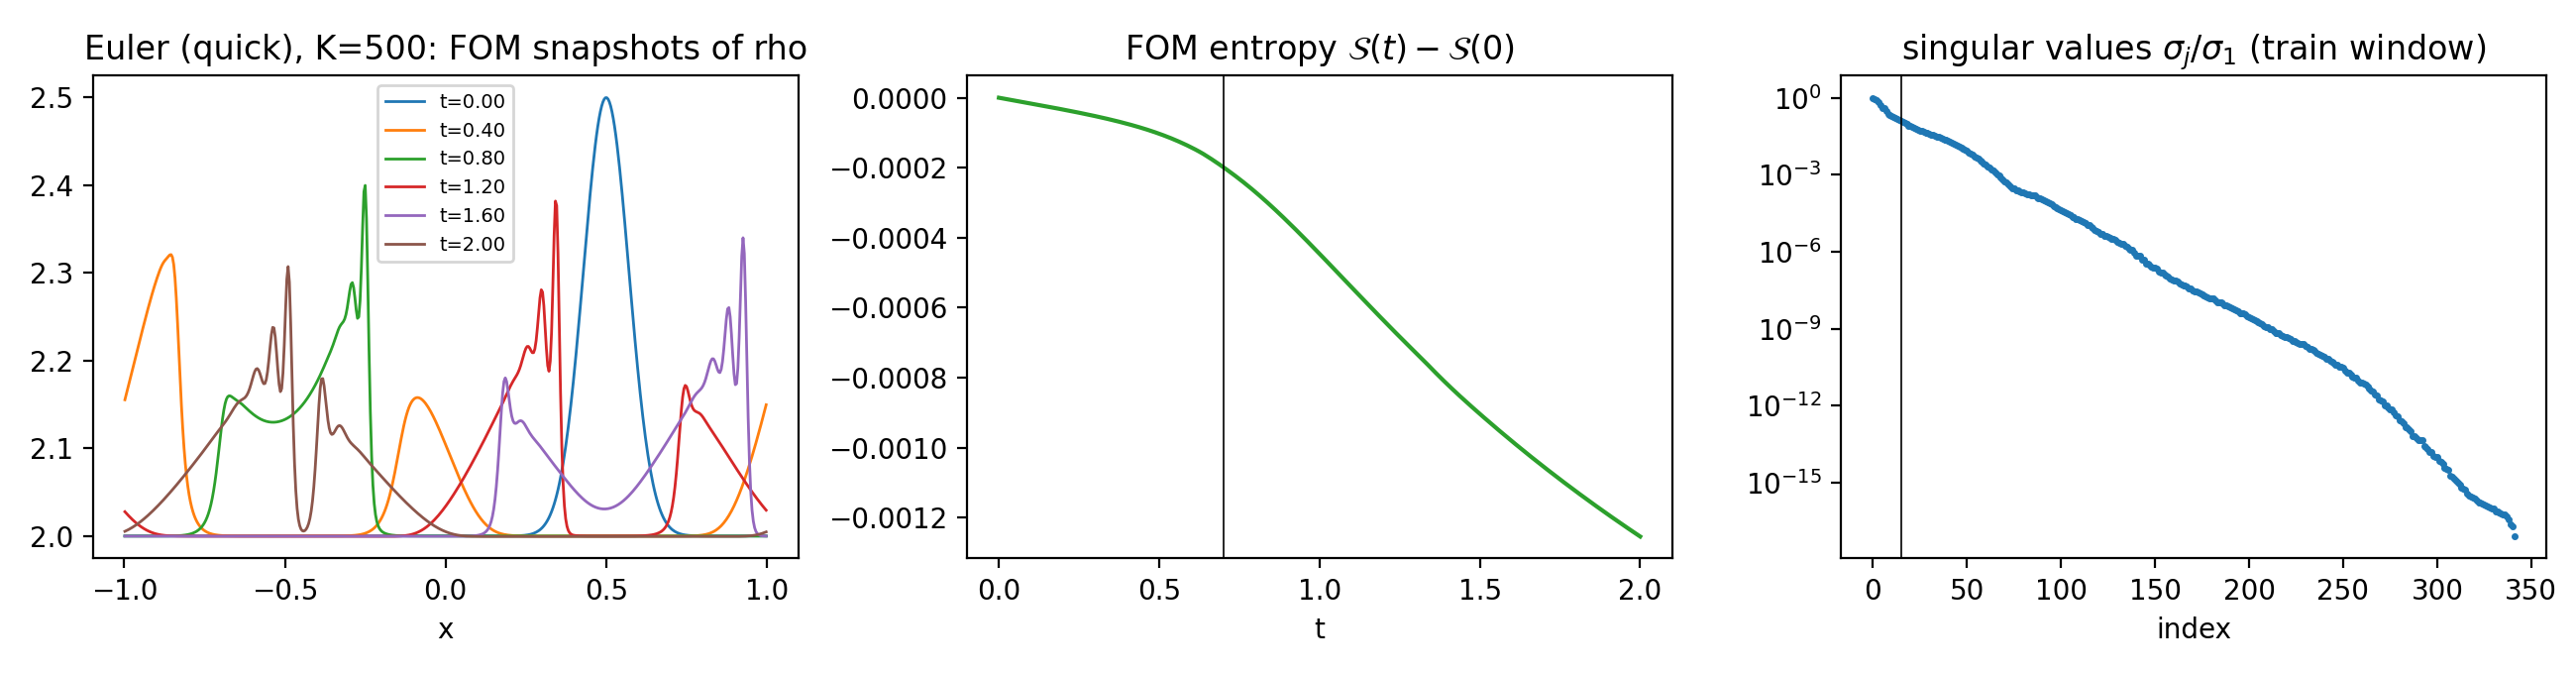
\includegraphics[width=\textwidth]{figs/fom_euler_quick.png}
\caption{FOM data. Left: snapshots. Middle: total entropy (the line marks $T_{\rm train}$). Right: snapshot singular values of the training window (the line marks $r=16$).}\label{fig:fom}
\end{figure}

%======================================================================
\section{Reduced space and the ES-ROM teacher}\label{sec:reduced}
%======================================================================

\subsection{POD basis with the constant mode}
\code{build\_basis} (\code{utils/pod.py:11}) builds the basis in four steps:
\begin{enumerate}
\item stack the snapshots of all conserved variables and, with \code{ENTROPY\_ENRICH}, of the entropy variables $v(u)$, as columns of one $K$-row matrix;
\item remove their component along $\mathbf 1/\sqrt K$;
\item take an SVD;
\item set
\[ V=\big[\mathbf 1/\sqrt K,\ \text{first } r-1 \text{ left singular vectors}\big],\qquad V^TV=I. \]
\end{enumerate}
One basis is shared by all variables (Kronecker convention), so $a=[a_\rho,a_{\rho u},a_E]$ with $r$ entries each, and $u\approx Va$ per variable.

Because $V^TV=I$, the reduced mass matrix is $M=\Delta x\,I$, and the projected entropy variables are
\begin{equation}\label{eq:vN}
v_N(a)=V^Tv(Va).
\end{equation}
$M$ and $v_N$ come from the same inner product. This matters: it is what makes Eq.~\eqref{eq:identity} below exact.

\paragraph{Conserved coefficients.} Every column except the first sums to zero, so
\[ \Delta x\textstyle\sum_i(Va)_{c,i} = \Delta x\sqrt K\,a_{cr}. \]
Total mass, momentum and energy are therefore carried only by the first coefficient of each variable block, at indices $\{0,r,2r\}$ (\code{conserved\_indices}).

\subsection{The core identity}
For \emph{any} reduced dynamics $\dot a$, the entropy of the reconstructed state $\Sc(a)=\Delta x\sum_iS((Va)_i)$ changes as
\begin{equation}\label{eq:identity}
\frac{d\Sc}{dt}=\Delta x\,v(Va)^TV\dot a=\Delta x\,v_N(a)^T\dot a = v_N^TM\dot a .
\end{equation}
Entropy stability is therefore the single scalar condition $v_N^TM\dot a\le0$.

\subsection{Teacher: unreduced ES-ROM (Chan 2020, Theorem 2)}
\code{utils/esrom.py} implements
\[
\tilde v = VV^Tv(Va),\quad \tilde u=u(\tilde v),\qquad
\Delta x\,\dot a_{ES}=-V^T\big[2(Q\circ F(\tilde u))\mathbf 1+\epsilon K_{\rm lap}\tilde u\big]
= \Delta x\,V^T\mathrm{rhs}_{\rm FOM}(\tilde u).
\]
The entropy variables of $\tilde u$ are exactly $\tilde v=Vv_N$. The convective part therefore conserves $\Sc$, and the viscous part dissipates it. The cost per RHS evaluation is $O(K)$.

With \code{entropy\_projection=False}, the same class gives the plain POD--Galerkin ROM $\dot a=V^T\mathrm{rhs}_{\rm FOM}(Va)$, which is \emph{not} entropy stable. The teacher has three uses:
\begin{itemize}
\item a label generator for training (Sec.~\ref{sec:losses});
\item a baseline in post-processing;
\item a reference the structured network reproduces exactly for one choice of $(J,R)$.
\end{itemize}

%======================================================================
\section{Network architecture}\label{sec:arch}
%======================================================================

\subsection{Structured network (\code{StructuredNet}, \code{esnn\_model.py:141})}
Figure~\ref{fig:arch} shows the whole network; the steps are:
\begin{enumerate}
\item \textbf{Input.} The reduced state $a\in\mathbb R^n$ (and parameters $\mu$, not used yet), normalized as $(a-\bar a)/\sigma_a$ with training-data statistics. Time is \emph{not} an input: the dynamics are autonomous, which helps extrapolation in time.
\item \textbf{Trunk.} An MLP with 4 hidden layers of width 256, tanh activations, Xavier-normal weights and zero biases (\code{mlp}, line 96).
\item \textbf{Output.} A vector $z\in\mathbb R^{n_J+n_L}$ of unconstrained numbers, where $n_f=n-n_{var}$ is the number of non-conserved coefficients:
\[ n_J = \tfrac{n_f(n_f-1)}{2},\qquad n_L=\tfrac{n_f(n_f+1)}{2}\ \ (\text{or } n_fk \text{ for a thin } L). \]
\item \textbf{Arrangement} (\code{factors}, line 172). $z_{1:n_J}$ fills a strictly upper-triangular $U$ (\code{torch.triu\_indices}). $z_{n_J+1:}$ fills a lower-triangular $L$ (\code{torch.tril\_indices}).
\item \textbf{Operators.} $J=D(U-U^T)D$ is skew-symmetric and $R=D\,LL^TD$ is positive semi-definite, where $D=\mathrm{diag}(d_1,\dots,d_{n_f})$ is a fixed \emph{per-mode scaling}. It is set from data before training (line 263) and is not trained:
\[ d_i^2=\Delta x\,\mathrm{rms}(\dot a_i)\,/\,\mathrm{rms}(v_i). \]
With this choice, an $O(1)$ diagonal entry of $U$ or $LL^T$ gives mode $i$ its own typical rate of change. For Burgers, $d_i$ runs from 0.03 (mode 1) to 0.50 (mode 15). The congruence $D(\cdot)D$ keeps skewness and semi-definiteness (Sec.~\ref{sec:es}); scaling one side only ($DJ$) would not. The $L$ rows of the last layer are multiplied by $l_{\rm init}=10^{-2}$, so $R$ starts small (plan: ``start nearly entropy conservative'').

\emph{Why per-mode.} The first version used one scalar $s$ ($J=s(U-U^T)$). For Burgers the mode amplitudes span five orders of magnitude ($4.6$ to $1.5\times10^{-5}$), so one scalar cannot make $O(1)$ outputs fit all modes. After training, the small modes had derivative errors of 30--3200\% and drifted out of the training range within $t\approx0.02$.
\item \textbf{Output dynamics} (\code{forward}, line 191): with $w=Dv_f$,
\[ \dot a_f = \frac{1}{\Delta x}\,D\big[(Uw-U^Tw)-L(L^Tw)\big],\qquad \dot a_c = 0, \]
where $v_f$ is the free part of $v_N(a)$. $J$ and $R$ are never formed in the forward pass; \code{operators()} forms them only for diagnostics.
\end{enumerate}


\begin{figure}[h]\centering
\resizebox{\textwidth}{!}{%
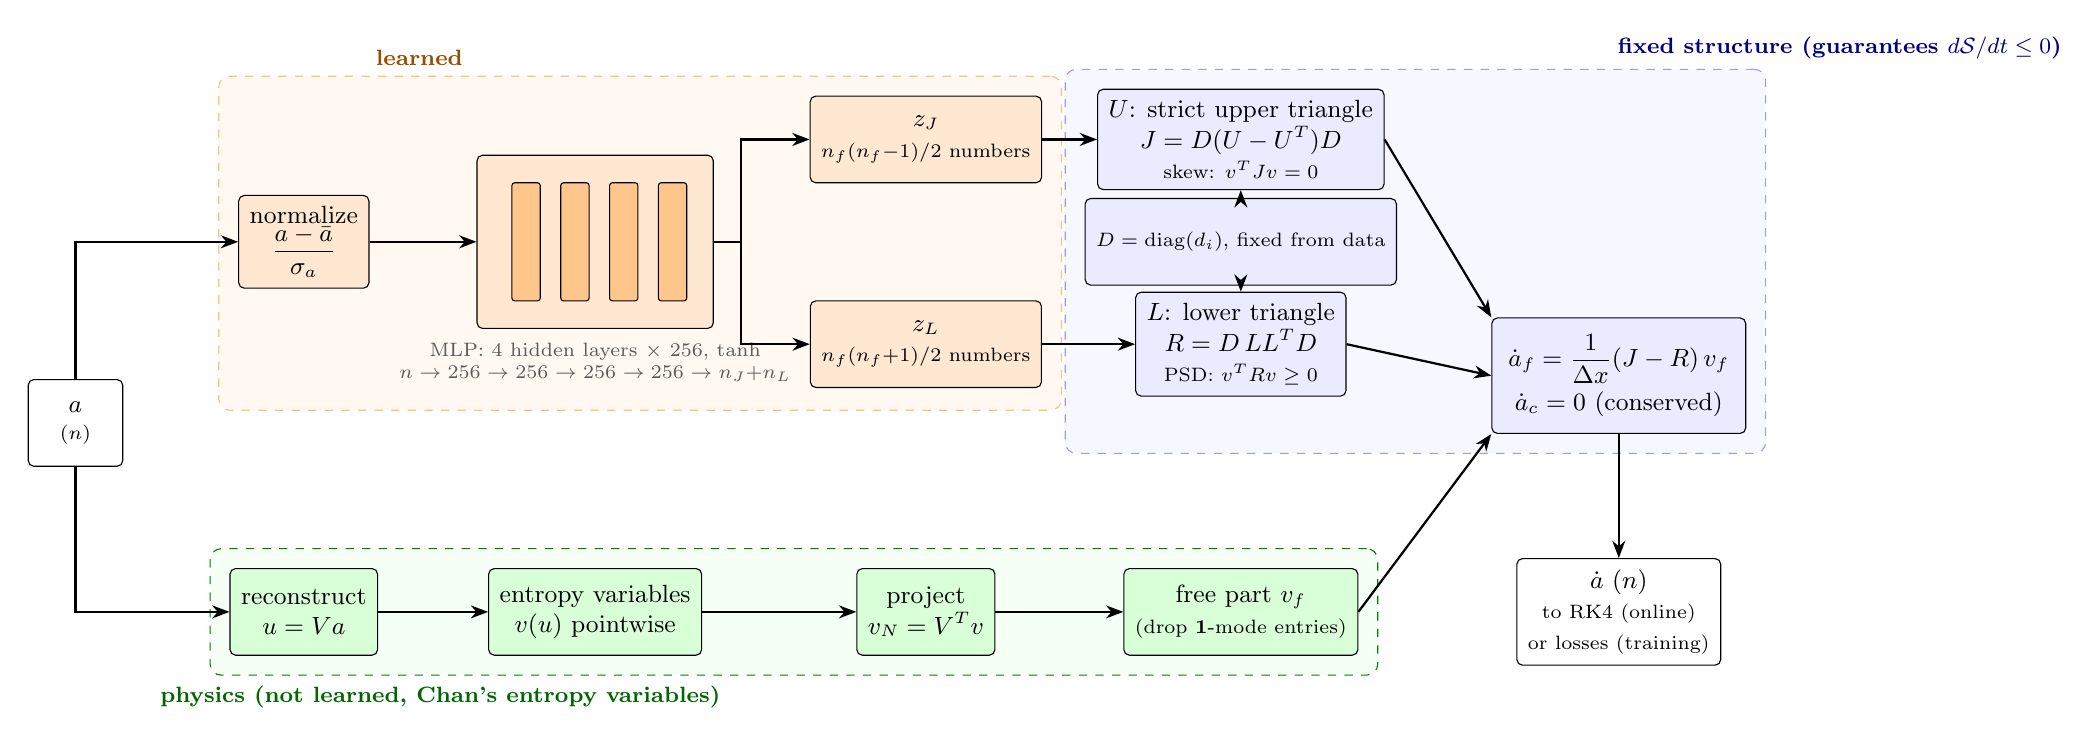
\begin{tikzpicture}[
  font=\small,
  box/.style={draw,rounded corners=2pt,align=center,inner sep=4pt,minimum height=11mm},
  learn/.style={box,fill=orange!18},
  phys/.style={box,fill=green!15},
  fixed/.style={box,fill=blue!8},
  arr/.style={-{Stealth[length=2.2mm]},thick},
  dim/.style={font=\scriptsize,text=black!65,align=center}]
% input
\node[box,fill=white,minimum width=12mm] (a) at (0,0) {$a$\\[-1pt]\scriptsize $(n)$};
% learned branch
\node[learn] (norm) at (2.9,2.3) {normalize\\$\dfrac{a-\bar a}{\sigma_a}$};
\node[learn,minimum width=30mm,minimum height=22mm] (mlp) at (6.6,2.3) {};
\foreach \k in {0,1,2,3} {
  \draw[fill=orange!45,rounded corners=1pt] ($(mlp.west)+(0.45+0.62*\k,-0.75)$) rectangle ++(0.36,1.5);
}
\node[dim,below=0.5mm of mlp.south] (mlpl) {MLP: 4 hidden layers $\times$ 256, tanh\\$n\to256\to256\to256\to256\to n_J{+}n_L$};
\node[learn] (zJ) at (10.8,3.6) {$z_J$\\\scriptsize $n_f(n_f{-}1)/2$ numbers};
\node[learn] (zL) at (10.8,1.0) {$z_L$\\\scriptsize $n_f(n_f{+}1)/2$ numbers};
\node[fixed] (J) at (14.8,3.6) {$U$: strict upper triangle\\$J=D(U-U^T)D$\\\scriptsize skew: $v^TJv=0$};
\node[fixed] (R) at (14.8,1.0) {$L$: lower triangle\\$R=D\,LL^TD$\\\scriptsize PSD: $v^TRv\ge0$};
\node[fixed,font=\scriptsize] (D) at (14.8,2.3) {$D=\mathrm{diag}(d_i)$, fixed from data};
% physics branch
\node[phys] (u)  at (2.9,-2.4) {reconstruct\\$u=Va$};
\node[phys] (v)  at (6.6,-2.4) {entropy variables\\$v(u)$ pointwise};
\node[phys] (vN) at (10.8,-2.4) {project\\$v_N=V^Tv$};
\node[phys] (vf) at (14.8,-2.4) {free part $v_f$\\\scriptsize (drop $\mathbf 1$-mode entries)};
% combine and output
\node[fixed,inner sep=6pt] (comb) at (19.6,0.6) {$\dot a_f=\dfrac{1}{\Delta x}(J-R)\,v_f$\\[2pt]$\dot a_c=0$ (conserved)};
\node[box,fill=white] (out) at (19.6,-2.4) {$\dot a$ $(n)$\\\scriptsize to RK4 (online)\\\scriptsize or losses (training)};
% arrows
\draw[arr] (a) |- (norm);
\draw[arr] (a) |- (u);
\draw[arr] (norm) -- (mlp);
\draw[arr] (mlp.east) -- ++(0.35,0) |- (zJ);
\draw[arr] (mlp.east) -- ++(0.35,0) |- (zL);
\draw[arr] (zJ) -- (J);
\draw[arr] (zL) -- (R);
\draw[arr] (D) -- (J);
\draw[arr] (D) -- (R);
\draw[arr] (u) -- (v);
\draw[arr] (v) -- (vN);
\draw[arr] (vN) -- (vf);
\draw[arr] (J.east) -- (comb.north west);
\draw[arr] (R.east) -- (comb.west);
\draw[arr] (vf.east) -- (comb.south west);
\draw[arr] (comb) -- (out);
% background bands
\begin{scope}[on background layer]
  \node[fit=(norm)(mlp)(mlpl)(zJ)(zL),fill=orange!5,draw=orange!50,dashed,rounded corners,inner sep=7pt,label={[font=\footnotesize\bfseries,text=orange!60!black]above left:learned}] {};
  \node[fit=(u)(v)(vN)(vf),fill=green!4,draw=green!50!black,dashed,rounded corners,inner sep=7pt,label={[font=\footnotesize\bfseries,text=green!40!black]below left:physics (not learned, Chan's entropy variables)}] {};
  \node[fit=(J)(R)(D)(comb),fill=blue!3,draw=blue!40,dashed,rounded corners,inner sep=7pt,label={[font=\footnotesize\bfseries,text=blue!50!black]above right:fixed structure (guarantees $d\mathcal S/dt\le0$)}] {};
\end{scope}
\end{tikzpicture}}
\caption{Structured network. The MLP (orange) only produces unconstrained numbers $z$. The fixed structure (blue) turns them into a skew $J$ and a positive semi-definite $R$, with the per-mode scaling $D$. The physics branch (green) computes the entropy variables of the reconstructed state. Their product gives $\dot a$ with $d\mathcal S/dt=-\|L^TDv_f\|^2\le0$ for any weights. Sizes for Euler: $n=48$, $n_f=45$, $n_J+n_L=2025$.}\label{fig:arch}
\end{figure}

\begin{table}[h]\centering
\caption{Network sizes with the default \code{NET} settings.}
\begin{tabular}{lcccccc}
\toprule
case & $n$ & $n_f$ & $n_J$ & $n_L$ & structured weights & unconstrained weights\\\midrule
Burgers & 16 & 15 & 105 & 120 & 259\,553 & 205\,840\\
Euler & 48 & 45 & 990 & 1035 & 730\,345 & 222\,256\\
\bottomrule
\end{tabular}
\end{table}

\subsection{Unconstrained baseline (\code{UnconstrainedNet}, line 202)}
The same trunk outputs $\dot a\in\mathbb R^n$ directly, scaled by the RMS of $\dot a$ in each variable block. It has no entropy structure and no conservation: it is the plain neural-ODE ROM the structured model is compared against.

\subsection{Closure model: ES-ROM + learned eddy viscosity (\code{ClosureNet}, line 214)}\label{sec:closure}
The structured network learns the \emph{whole} reduced dynamics. The closure model keeps Chan's operators exact and learns only what the truncated ROM misses:
\begin{equation}\label{eq:closure}
\dot a=\dot a_{ES}(a)\;-\;V^TD^T\big(\nu_\theta\odot D\tilde u\big),\qquad
\nu_\theta(x;a)=\nu_0\,\mathrm{softplus}\Big(z_0(a)+\textstyle\sum_{k=1}^{m}z_k(a)\,\phi_k(x)\Big)\;\ge0 .
\end{equation}
\begin{itemize}
\item \textbf{The terms.}
  \begin{itemize}
  \item $\dot a_{ES}$ is the unreduced ES-ROM (Sec.~\ref{sec:reduced}).
  \item $D$ is the edge difference $(D u)_{i+1/2}=(u_{i+1}-u_i)/\Delta x$, the same as in the FOM viscosity.
  \item $\tilde u=u(Vv_N)$ is the entropy-projected state of the ES-ROM.
  \item $\phi_k$ are the non-constant POD modes evaluated at the cell edges, so the viscosity can concentrate where the solution has structure.
  \item $\nu_0$ is the FOM viscosity $\epsilon$.
  \end{itemize}
\item \textbf{Network.} The MLP (same trunk as before) maps $a$ to only $m+1=r$ numbers $z$. Everything else is fixed physics.
\item \textbf{Entropy.} The closure changes the entropy by
\[ \Delta x\,v_N^T\dot a_{\mathbb C}=-\Delta x\sum_e\nu_e\,(D\tilde v)_e^T(D\tilde u)_e\le0, \]
because $\tilde v=Vv_N$ are the entropy variables of $\tilde u$ and $u(v)$ is monotone. This is the same argument as for the FOM viscosity, edge by edge. Added to the entropy stable ES-ROM, the model is entropy stable for any weights.
\item \textbf{Conservation and free stream.} The closure is a difference of edge fluxes, so the totals are conserved. For a uniform state $D\tilde u=0$, so it vanishes.
\item \textbf{Training.}
  \begin{itemize}
  \item Losses: data loss and entropy-rate loss only. The teacher loss is switched off, because the base model \emph{is} the teacher.
  \item Initialization: at $z_0=-3$ the model starts as the ES-ROM ($\nu\approx0.05\epsilon$).
  \item Precomputed once: $\dot a_{ES}$ and $D\tilde u$ at the training states, since they do not depend on the weights.
  \end{itemize}
\end{itemize}

%======================================================================
\section{How entropy stability is constructed}\label{sec:es}
%======================================================================
Substituting the structured output into the identity \eqref{eq:identity}, using $\dot a_c=0$ and writing $w=Dv_f$:
\begin{equation}
\frac{d\Sc}{dt}=\Delta x\,v_N^T\dot a
= \underbrace{\big(w^TUw - w^TU^Tw\big)}_{=0\ \text{(a scalar equals its transpose)}} \;-\; \underbrace{w^TLL^Tw}_{=\|L^Tw\|^2}
= -\|L^TDv_f\|^2\ \le\ 0 .
\end{equation}
This holds for \emph{every} state $a$ and \emph{every} set of weights. Training cannot break it, and no loss term is needed to enforce it. Four properties support it:
\begin{enumerate}
\item \textbf{$v_N$ is physics, not learned} (\code{ReducedNet.v\_N}, line 132). If $v_N$ were learned, the bound would hold for a fake entropy.
\item \textbf{Same inner product.} $M=\Delta xI$ and $v_N=V^Tv(Va)$ both follow from $V^TV=I$. Hyper-reduction (plan phase 3) must change both together.
\item \textbf{$D$ is a fixed buffer, not a trainable weight.} Any $D$ keeps the bound, but a trainable $d_i$ could collapse to 0 and switch mode $i$ off.
\item \textbf{Conservation.} The conserved rows and columns of $J$ and $R$ are removed by building $U$ and $L$ only on the $n_f$ free coefficients. This is equivalent to the plan's mask $\Pi_cJ\Pi_c$, with $n_f^2$ instead of $n^2$ outputs. Since $\dot a_c=0$ exactly, total mass, momentum and energy are constant.
\end{enumerate}
\paragraph{Generality.} No expressiveness is lost. Any entropy conservative field $f$ ($v^Tf=0$) equals $Jv$ for the skew matrix $J=(fv^T-vf^T)/\|v\|^2$. Chan's ES-ROM is itself one $(J,R)$ pair. $J$ plays the role of the flux-differencing term $2V^T(Q\circ F)\mathbf 1$, and $R$ the role of the viscosity.

\subsection{Where Chan's zero row sum property $Q\mathbf 1=0$ lives}\label{sec:rowsum}
In Chan (2020), $Q$ must be skew-symmetric \emph{and} satisfy $Q\mathbf 1=0$. Skew-symmetry together with $Q\mathbf 1=0$ gives three things:
\begin{enumerate}
\item[(a)] \textbf{Entropy conservation.} The $\psi$ terms of the shuffle condition cancel: $\psi^TQ\mathbf 1-\mathbf 1^TQ\psi=0$.
\item[(b)] \textbf{Conservation.} $\mathbf 1^TQ=0$.
\item[(c)] \textbf{Consistency.} A uniform state is steady, because $F_{ij}=f(u)$ gives $(Q\circ F)\mathbf 1=f(u)\,Q\mathbf 1=0$.
\end{enumerate}
In the hyper-reduced ROM the property is \emph{not} automatic. It is the reason the test basis must contain $\mathbf 1$ (Lemma 1, $Q_t\mathbf 1=0$), as implemented in \code{FOM/esrom/rom.py} (\code{test\_basis}, $[\mathbf 1,V,QV]$). This code has no hyper-reduction. Below is where the property is used, layer by layer.

\begin{center}\small
\begin{tabular}{p{2.5cm}p{7.6cm}p{4.9cm}}
\toprule
layer & how $Q\mathbf 1=0$ is enforced or replaced & measured, see\newline\code{logs/zero\_row\_sum\_check.log}\\\midrule
FOM\newline\code{utils/fom.py}\newline line 62 & $Q$ is never formed. \code{conv} uses $f_S(u_i,u_{i+1})-f_S(u_{i-1},u_i)$, i.e.\ row $i$ of $Q$ is $(-\tfrac12,0,+\tfrac12)$: zero row sum \emph{by construction} (the stencil). (a)--(c) hold exactly. & row sums of the implicit $Q$: $0$; $\mathrm{rhs}$ of a uniform state: $0$ (exact)\\
teacher ES-ROM\newline\code{utils/esrom.py}\newline line 38 & Unreduced: it calls the FOM \code{conv} on $\tilde u$, so it inherits the full-order $Q$. Chan's Theorem 2 conservation condition $\mathbf 1\in\mathrm{range}(V)$ holds because $V_{:,0}=\mathbf 1/\sqrt K$ (\code{utils/pod.py:11}). & $|\dot a_{ES}|$ at a uniform state: $4\times10^{-14}$\\
structured network\newline\code{esnn\_model.py}\newline line 191 & There is no $Q$ and no two-point flux, so no row-sum condition is needed. Each role is taken over by structure: (a) $\to$ skewness of $J$ alone ($v^TJv=0$ needs no $\psi$ telescoping); (b) $\to$ zero conserved rows/columns of $J,R$ ($\dot a_c=0$), the analogue of $\mathbf 1^TQ=0$, since $\mathbf 1^TV\dot a=\sqrt K\dot a_0$; (c) $\to$ for a uniform state $u$, $v(u)$ is uniform and the non-constant modes sum to zero, so $v_f=0$ and hence $\dot a=0$ for \emph{any} weights. & random weights: $|\dot a|=8\times10^{-14}$ at a uniform state (vs.\ $4.1$ on snapshots); unconstrained net: $1.4$\\
\bottomrule
\end{tabular}
\end{center}
So the network has no explicit zero row sum restriction. The property is replaced by two features: the constant mode is the first basis vector, and the free coefficients carry $v_f$. Uniform states are therefore exact steady states of the structured network (``free-stream preservation''). The unconstrained baseline does not have this property.

\paragraph{What is \emph{not} guaranteed.}
\begin{itemize}
\item \textbf{The time-stepping.} The bound is semi-discrete. RK4 may change the entropy by $O(\Delta t^5)$ per step; relaxation RK would remove this.
\item \textbf{Positivity.} If $\rho\le0$ or $p\le0$ somewhere in $Va$, then $v_N$ is NaN and the rollout stops. Chan's ES-ROM has the same limitation.
\item \textbf{Accuracy.} Accuracy comes from the losses, not from the structure.
\end{itemize}

%======================================================================
\section{How the pieces are coupled}\label{sec:coupling}
%======================================================================

\begin{figure}[h]\centering
\resizebox{\textwidth}{!}{%
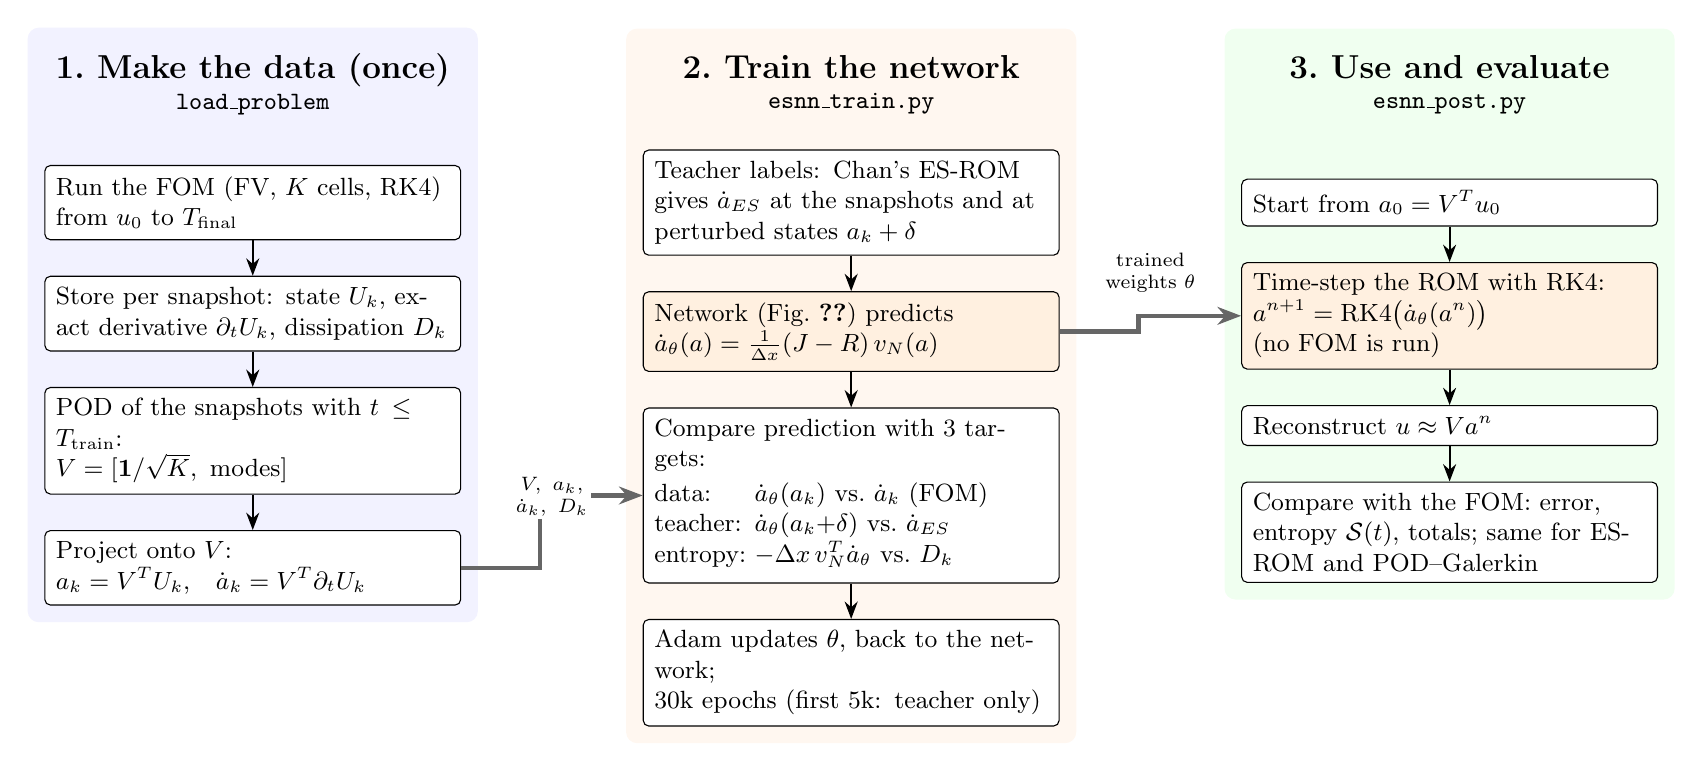
\begin{tikzpicture}[
  font=\small,
  stp/.style={draw,rounded corners=2pt,align=left,text width=50mm,inner sep=4pt,fill=white},
  num/.style={circle,draw,fill=black,text=white,font=\scriptsize\bfseries,inner sep=1pt,minimum size=4.2mm},
  arr/.style={-{Stealth[length=2.2mm]},thick},
  big/.style={-{Stealth[length=3mm]},line width=1.6pt,black!60},
  head/.style={font=\bfseries,align=center}]
% ---- column 1: data
\node[head] (h1) at (0,0.2) {\large 1.\ Make the data (once)\\[-1pt]\normalsize\code{load\_problem}};
\node[stp] (s1) at (0,-1.3) {Run the FOM (FV, $K$ cells, RK4)\\from $u_0$ to $T_{\rm final}$};
\node[stp] (s2) [below=4.5mm of s1] {Store per snapshot: state $U_k$, exact derivative $\partial_tU_k$, dissipation $D_k$};
\node[stp] (s3) [below=4.5mm of s2] {POD of the snapshots with $t\le T_{\rm train}$:\\$V=[\mathbf 1/\sqrt K,\ \text{modes}]$};
\node[stp] (s4) [below=4.5mm of s3] {Project onto $V$:\\$a_k=V^TU_k$,\quad $\dot a_k=V^T\partial_tU_k$};
% ---- column 2: training
\node[head] (h2) at (7.6,0.2) {\large 2.\ Train the network\\[-1pt]\normalsize\code{esnn\_train.py}};
\node[stp] (t1) at (7.6,-1.3) {Teacher labels: Chan's ES-ROM gives $\dot a_{ES}$ at the snapshots and at perturbed states $a_k+\delta$};
\node[stp,fill=orange!12] (t2) [below=4.5mm of t1] {Network (Fig.~\ref{fig:arch}) predicts\\$\dot a_\theta(a)=\tfrac1{\Delta x}(J-R)\,v_N(a)$};
\node[stp] (t3) [below=4.5mm of t2] {Compare prediction with 3 targets:\\[2pt]
\begin{tabular}{@{}l@{\ }l@{}}
data: & $\dot a_\theta(a_k)$ vs.\ $\dot a_k$ (FOM)\\
teacher: & $\dot a_\theta(a_k{+}\delta)$ vs.\ $\dot a_{ES}$\\
entropy: & $-\Delta x\,v_N^T\dot a_\theta$ vs.\ $D_k$
\end{tabular}};
\node[stp] (t4) [below=4.5mm of t3] {Adam updates $\theta$, back to the network;\\30k epochs (first 5k: teacher only)};
% ---- column 3: online
\node[head] (h3) at (15.2,0.2) {\large 3.\ Use and evaluate\\[-1pt]\normalsize\code{esnn\_post.py}};
\node[stp] (o1) at (15.2,-1.3) {Start from $a_0=V^Tu_0$};
\node[stp,fill=orange!12] (o2) [below=4.5mm of o1] {Time-step the ROM with RK4:\\$a^{n+1}=\mathrm{RK4}\big(\dot a_\theta(a^n)\big)$\\(no FOM is run)};
\node[stp] (o3) [below=4.5mm of o2] {Reconstruct $u\approx Va^n$};
\node[stp] (o4) [below=4.5mm of o3] {Compare with the FOM: error, entropy $\mathcal S(t)$, totals; same for ES-ROM and POD--Galerkin};
% ---- arrows within columns
\foreach \x/\y in {s1/s2,s2/s3,s3/s4,t1/t2,t2/t3,t3/t4,o1/o2,o2/o3,o3/o4} \draw[arr] (\x) -- (\y);
% ---- arrows between columns (horizontal)
\draw[big] (s4.east) -- ++(1.0,0) |- (t3.west);
\node[font=\scriptsize,align=center,fill=white,inner sep=1pt] at ($(s4.east)!0.5!(s4.east -| t3.west)+(0,0.9)$) {$V,\ a_k,$\\$\dot a_k,\ D_k$};
\draw[big] (t2.east) -- ++(1.0,0) |- (o2.west);
\node[font=\scriptsize,align=center,fill=white,inner sep=1pt] at ($(t2.east)!0.5!(t2.east -| o2.west)+(0,0.75)$) {trained\\weights $\theta$};
% ---- column backgrounds
\begin{scope}[on background layer]
\node[fit=(h1)(s1)(s4),fill=blue!5,rounded corners,inner sep=6pt] {};
\node[fit=(h2)(t1)(t4),fill=orange!6,rounded corners,inner sep=6pt] {};
\node[fit=(h3)(o1)(o4),fill=green!6,rounded corners,inner sep=6pt] {};
\end{scope}
\end{tikzpicture}}
\caption{The three stages, read left to right and top to bottom. Stage 1 runs the FOM once and turns it into reduced data. Stage 2 fits the network's $\dot a_\theta$ to three targets. Stage 3 uses only the trained network to march in time, then compares with the FOM. Orange boxes are where the network is used.}\label{fig:coupling}
\end{figure}

\subsection{Offline (\code{esnn\_train.py})}
\begin{enumerate}
\item \code{load\_problem}: run the FOM (or load the cache) and build $V$ from snapshots with $t\le T_{\rm train}$.
\item \code{ReducedProblem}: project the data to $a_k$ and $\dot a_k$, and create the teacher and POD--Galerkin ROMs on the same $V$.
\item Sanity prints before training: $\|V^TV-I\|$, the projection error at $T_{\rm train}$ and $T_{\rm final}$, the teacher's convective entropy residual, and $\max d\Sc/dt$ of the teacher.
\item \code{ESNNROM.\_\_init\_\_} prepares training:
  \begin{itemize}
  \item collect the training samples;
  \item build the teacher samples;
  \item precompute $v_N$ at all fixed inputs (it is constant during training, so it is never recomputed);
  \item set the input normalization, the per-mode scaling $D$ and the loss scales.
  \end{itemize}
\item \code{train}: Adam with $\mathrm{lr}=10^{-3}$ and \code{StepLR(5000, 0.9)}. It saves \code{weights.pt}, \code{weights\_best.pt}, the loss history, \code{loss.png} and \code{report.txt}.
\end{enumerate}

\subsection{Training losses}\label{sec:losses}
\begin{description}
\item[Data] $\displaystyle L_{data}=\frac1{n_{var}}\sum_c\frac{\mathrm{mean}_k\|\dot a_{\theta,c}(a_k)-\dot a_{k,c}\|^2}{\mathrm{mean}_k\|\dot a_{k,c}\|^2}$, over the FOM snapshots in the training window ($c$ = variable block). This is the ground truth: it contains the effect of the truncated modes.
\item[Teacher] The same form, on the snapshots plus \code{n\_teacher} Gaussian perturbations $a_k+\delta$, with target $\dot a_{ES}$. The perturbation has std $0.1\times$ that of each coefficient, and conserved coefficients are not perturbed. Inadmissible states are dropped. This term covers states off the trajectory, which the rollout will visit.
\item[Entropy rate] $L_{ent}=\mathrm{mean}_k(D_\theta-D_k)^2/\mathrm{mean}_kD_k^2$ with $D_\theta=-\Delta x\,v_N^T\dot a_\theta$ ($=v_f^TRv_f$ for the structured net). The target $D_k$ is $\epsilon v^TK_{\rm lap}u$ from the FOM (default), or the rate of the projected data. This term stops the model from damping too much or too little.
\item[Schedule] For the first \code{n\_pretrain} epochs only $L_{teacher}$ is used, so the model starts close to the ES-ROM. After that, the loss is $L=L_{data}+L_{teacher}+0.1\,L_{ent}$.
\end{description}

\subsection{Online (\code{esnn\_post.py})}
\begin{itemize}
\item \textbf{Rollout.} Start from $a_0=V^Tu_0$ and integrate $\dot a=\mathrm{net}(a)$ with the same RK4 and $\Delta t$ as the FOM, saving at the FOM snapshot times. The rollout stops at the first non-finite state.
\item \textbf{Models compared.} The structured network, the unconstrained network, the ES-ROM teacher and POD--Galerkin.
\item \textbf{Metrics.} Relative $L^2$ error of $Va$ against the FOM, compared with the projection error (the best any ROM in $\mathrm{span}(V)$ can do); $\Sc(t)$; $-d\Sc/dt$; drift of the conserved totals; admissibility; wall time per step; and $\max|v^TJv|$ along the trained trajectory.
\end{itemize}

\subsection{Code map}
\begin{center}\small
\begin{tabular}{p{4.4cm}p{11.2cm}}
\toprule
Location & Role\\\midrule
\code{esnn\_config.py} & case table, \code{NET}, \code{TRAIN}, device, seed; environment switches \code{ESNN\_PROBLEM/MODEL/QUICK/DEVICE}\\
\code{utils/physics.py} & $S$, $v$, $u(v)$, $f$, $f_S$, $\psi$, log mean, admissibility\\
\code{utils/fom.py} & \code{FOM1D} (conv 62, visc 67, rhs 71), RK4 (27, 36), \code{generate\_snapshots} (100)\\
\code{utils/pod.py} & \code{build\_basis} (11), \code{project}/\code{reconstruct}, \code{conserved\_indices}\\
\code{utils/esrom.py} & \code{ESROM}: \code{v\_N} (28), \code{states} (32), \code{rhs} (38), \code{entropy\_residual}, \code{entropy\_rate}\\
\code{esnn\_model.py} 29--87 & \code{make\_fom}, \code{ReducedProblem}, \code{load\_problem} (cache)\\
\code{esnn\_model.py} 96--272 & \code{mlp}, \code{ReducedNet} ($v_N$ 132), \code{StructuredNet} (factors 172, operators 185, forward 191), \code{UnconstrainedNet} (202), \code{ClosureNet} (214: viscosity 241, closure 252, forward 257), \code{build\_net} (262)\\
\code{esnn\_model.py} 275--465 & \code{ESNNROM}: samples, teacher switch (305), $D$ (321), closure cache (328), \code{teacher\_samples} (349), losses (365--376), \code{loss\_func} (377), \code{train} (423)\\
\code{esnn\_model.py} 471--486 & \code{net\_rhs}, \code{rollout}\\
\code{esnn\_train.py}, \code{esnn\_post.py} & drivers (Sec.~\ref{sec:coupling})\\
\code{tests/} & four test files, \code{helpers.py} (small FOM runs), \code{run\_tests.py} (runner)\\
\bottomrule
\end{tabular}
\end{center}

%======================================================================
\section{Unit tests}\label{sec:tests}
%======================================================================

\paragraph{Procedure.} pytest is not installed in this environment, and nothing was installed. Instead, a small runner (\code{tests/run\_tests.py}) imports one test file and runs each \code{test\_*} function separately. It times each test and continues after a failure.
\begin{itemize}
\item \textbf{One file at a time}, in the order physics $\to$ FOM $\to$ basis/teacher $\to$ network, each run with \code{python tests/run\_tests.py tests/<file>}.
\item \textbf{Logs} are in \code{report/logs/}.
\item \textbf{Measured values.} The tests only check thresholds, so the value each invariant actually reaches was measured separately (\code{report/measure\_invariants.py}, \code{report/logs/measurements.json}). These are the numbers in the tables below.
\item \textbf{Problem sizes.} All tests use small problems on the CPU: Euler with $K=100$--200 and $r=6$ ($n=18$), and Burgers with $K=100$ and $r=6$.
\end{itemize}

\begin{table}[h]\centering
\caption{Summary.}
\begin{tabular}{lccc}
\toprule
file & tests & result & time\\\midrule
\code{test\_physics.py} & 8 & 8/8 \pass\ (after fixing one test reference) & 1.6 s\\
\code{test\_fom.py} & 6 & 6/6 \pass & 0.9 s\\
\code{test\_pod\_esrom.py} & 8 & 8/8 \pass & 3.6 s\\
\code{test\_model.py} & 11 & 11/11 \pass & 13 s\\\midrule
total & 33 & 33/33 & $\approx$20 s\\
\bottomrule
\end{tabular}
\end{table}

\subsection{\code{test\_physics.py}: physics functions}\label{sec:t-physics}
Random admissible states: 1000 per check for the measurements, 100 in the tests.
\begin{center}\small
\begin{tabular}{p{4.3cm}p{5.0cm}p{3.9cm}c}
\toprule
test & checks & measured (Burgers / Euler) & result\\\midrule
\code{entropy\_vars\_are\_gradient\_of\_entropy} & $v(u)=\nabla_uS$ via autograd & $0$ / $8.9\times10^{-16}$ & \pass\\
\code{round\_trip} & $u(v(u))=u$ & $0$ / $1.8\times10^{-14}$ & \pass\\
\code{flux\_properties} & consistency $f_S(u,u)=f(u)$; symmetry; shuffle $(v_L-v_R)^Tf_S=\psi_L-\psi_R$ & $8.9\times10^{-16}$ / $7.1\times10^{-15}$; $4.4\times10^{-16}$ / $7.1\times10^{-15}$; $1.8\times10^{-15}$ / $4.0\times10^{-15}$ & \pass\\
\code{flux\_nearly\_equal\_states} & shuffle for $|u_L-u_R|\sim10^{-9}$ (series branch of the log mean) & -- / $4.0\times10^{-15}$ & \pass\\
\code{psi\_is\_potential} & $\psi=v^Tf-F$ (scaling of $\psi$) & $1.8\times10^{-15}$ / $4.0\times10^{-15}$ & \pass\\
\code{logmean} & against an accurate reference, $|b/a-1|\in[10^{-12},10^{-1}]$ & rel.\ err.\ $4.4\times10^{-16}$ & \pass$^\ast$\\
\code{logmean\_gradient\_is\_finite} & $\partial\{\!\{a\}\!\}_{\log}/\partial a$ at $a=b$ is finite and $=\tfrac12$ & exact & \pass\\
\code{euler\_admissibility} & $\rho>0,\ p>0$ flags, batched & correct & \pass\\
\bottomrule
\end{tabular}
\end{center}
$^\ast$\textbf{The one failure, and its fix.} On the first run, \code{test\_logmean} \fail ed. The test's reference value was the naive formula $(a-b)/(\log a-\log b)$, which loses digits to cancellation when $a\approx b$. A 50-digit \code{mpmath} reference (\code{report/logs/logmean\_diagnosis.log}) showed:
\begin{itemize}
\item the code's log mean is accurate to $3.7\times10^{-16}$;
\item the naive reference has error $1.2\times10^{-9}$ at $|b/a-1|\sim10^{-6}$, just over the test's tolerance of $10^{-9}$.
\end{itemize}
The reference was changed to the cancellation-free $(a-b)/(-\mathrm{log1p}((b-a)/a))$, and the tolerance was tightened to $10^{-13}$. No code in \code{utils/} was changed.

\subsection{\code{test\_fom.py}: full order model}
Euler pulse with $K=200$; Burgers wave with $K=200$.
\begin{center}\small
\begin{tabular}{p{4.3cm}p{5.2cm}p{3.7cm}c}
\toprule
test & checks & measured & result\\\midrule
\code{conservation\_of\_totals} & $\sum_i\mathrm{rhs}_i=0$ (telescoping), $\epsilon>0$ & $1.4\times10^{-14}$ & \pass\\
\code{entropy\_conservative\_convection} & $v^T2(Q\circ F)\mathbf 1=0$ & $-5.9\times10^{-17}$ (scale 3.6) & \pass\\
\code{viscous\_dissipation\_nonnegative} & $D=\epsilon v^TKu\ge0$ and $\Delta x\,v^T\dot u=-D$ & $D=8.4\times10^{-4}$; mismatch $4.5\times10^{-17}$ & \pass\\
\code{batched\_rhs\_matches\_loop} & batched $(B,n_{var},K)$ evaluation = loop & identical & \pass\\
\code{matches\_numpy\_fv\_code} & RHS equals the committed FV code \code{FOM/esrom} & max diff.\ $2.0\times10^{-14}$ & \pass\\
\code{entropy\_drift\_converges\_with\_dt} & $\epsilon=0$: RK4 entropy drift $\to0$ & see below & \pass\\
\bottomrule
\end{tabular}
\end{center}
Entropy drift at $T=0.2$ with $\epsilon=0$ ($K=100$) for 50, 100, 200 and 400 steps: $1.2\times10^{-9}$, $6.0\times10^{-11}$, $3.2\times10^{-12}$ and $1.9\times10^{-13}$. The successive ratios are 20.5, 18.7 and 17.0, close to $2^4=16$. So the semi-discrete scheme conserves entropy, and the only drift is the 4th-order time error.

\subsection{\code{test\_pod\_esrom.py}: basis and teacher}
Euler with $K=100$, $\epsilon=10^{-3}$, snapshots to $t=0.3$, basis from $t\le0.2$, $r=6$ ($n=18$).
\begin{center}\small
\begin{tabular}{p{4.5cm}p{5.0cm}p{3.7cm}c}
\toprule
test & checks & measured & result\\\midrule
\code{basis\_orthonormal\_with\_constant\_mode} & $V^TV=I$; $V_{:,0}=1/\sqrt K$; other columns sum to 0; $\sigma$ sorted & $4.4\times10^{-16}$; exact; $5.6\times10^{-16}$ & \pass\\
\code{project\_reconstruct} & $V^T(Va)=a$ & round-off & \pass\\
\code{totals\_live\_in\_constant\_coefficients} & totals $=\Delta x\sqrt K\,a_{cr}$ & rel.\ $<10^{-12}$ & \pass\\
\code{teacher\_entropy\_conservative\_convection} & $|v_N^TV^T2(Q\circ F)\mathbf 1|$ at round-off (Chan Fig.~4) & rel.\ $7.5\times10^{-15}$ & \pass\\
\code{teacher\_entropy\_stable\_and\_conservative} & $d\Sc/dt\le0$; conserved rates $=0$ & $\max d\Sc/dt=-1.9\times10^{-4}$; $3.5\times10^{-15}$ & \pass\\
\code{teacher\_entropy\_conservative\_without\_viscosity} & $\epsilon=0$: $d\Sc/dt=0$ & $3.5\times10^{-16}$ & \pass\\
\code{burgers\_entropy\_projection\_is\_trivial} & $v=u$ $\Rightarrow$ ES-ROM $=$ Galerkin & $1.8\times10^{-14}$ & \pass\\
\code{projected\_data\_is\_consistent} & $\dot a_k=V^T\mathrm{rhs}(U_k)$; projection error $<1$ & error $1.2\times10^{-2}$ at $t=0.2$, $5.2\times10^{-2}$ at $t=0.3$ & \pass\\
\bottomrule
\end{tabular}
\end{center}
The projection error grows from $1.2\%$ at the end of the basis window to $5.2\%$ just $0.1$ later. This is a first sign of how fast this transport problem leaves a fixed POD space.

\subsection{\code{test\_model.py}: network structure and trainer}\label{sec:t-model}
Random (untrained) weights; small network (2 layers of width 32), with $l_{\rm init}=1$ so that $R$ is not small. Measurements use 64 admissible states near the snapshots.
\begin{center}\small
\begin{tabular}{p{4.3cm}p{4.8cm}p{4.1cm}c}
\toprule
test & checks & measured (full $L$ / rank-3 $L$) & result\\\midrule
\code{structured\_random\_weights\_euler} & $J=-J^T$; $\max\frac{|v^TJv|}{|v|^2\|J\|}$; $\lambda_{\min}(R)$; $d\Sc/dt=-v^TRv\le0$; $\dot a_c=0$ & $2.7\times10^{-17}$; $-1.6\times10^{-18}$ (rel.); $\max d\Sc/dt=-8.9\times10^{-4}$; mismatch $7\times10^{-16}$; exactly 0 & \pass\\
\code{structured\_low\_rank} & same with thin $L\in\mathbb R^{n_f\times3}$ & $2.6\times10^{-17}$; $-3.6\times10^{-16}$; $-2.1\times10^{-4}$; $4\times10^{-16}$; 0 & \pass\\
\code{output\_sizes} & $n_f$, $n_J$, $n_L$; baseline output shape & as Sec.~\ref{sec:arch} & \pass\\
\code{precomputed\_vN\_matches} & \code{forward(a, vN=...)} $=$ \code{forward(a)} & identical & \pass\\
\code{batch\_consistency} & batched forward $=$ one state at a time & round-off & \pass\\
\code{rollout\_entropy\_nonincreasing\_burgers} & fully discrete RK4 rollout ($\Delta t=10^{-4}$, $t\le0.2$): $\Sc$ non-increasing, totals constant & every step decreases $\Sc$ (largest step change $-4.1\times10^{-7}$); totals drift $6.2\times10^{-17}$ & \pass\\
\code{trainer\_smoke} & 4 epochs (2 pretrain) for both networks: finite losses; structure intact after updates & see below & \pass\\
\code{closure\_entropy\_and\_conservation} & closure (Sec.~\ref{sec:closure}), random weights, Euler: $\nu\ge0$; closure $d\Sc/dt<0$; total $d\Sc/dt\le0$; conserved rates & all $\le$ round-off (rel.\ $10^{-12}$--$10^{-13}$) & \pass\\
\code{closure\_reduces\_to\_esrom\_and\_keeps\_uniform\_states} & $\nu=0\Rightarrow$ exactly the ES-ROM; cached $=$ uncached; uniform state $\Rightarrow$ closure $=0$ & exact; round-off & \pass\\
\code{closure\_rollout\_entropy\_nonincreasing\_burgers} & RK4 rollout: $\Sc$ non-increasing; totals constant & as for the structured net & \pass\\
\code{closure\_trainer\_smoke} & 4 epochs: finite losses; no teacher samples; $\nu\ge0$ after updates & -- & \pass\\
\bottomrule
\end{tabular}
\end{center}

\paragraph{Untrained structured vs.\ unconstrained network.} Figure~\ref{fig:random} rolls out both untrained networks from the same Burgers initial state.
\begin{itemize}
\item \textbf{Structured net.} $\Sc$ decreases at every step ($0.5000\to0.4960$), and the totals stay constant to $6\times10^{-17}$.
\item \textbf{Unconstrained net.} $\Sc$ \emph{increases} ($0.5000\to0.5321$; the largest single-step increase is $+2.4\times10^{-4}$), and the total mass drifts by $6.7\times10^{-2}$.
\end{itemize}
This is the guarantee of Sec.~\ref{sec:es} working before any training.

\begin{figure}[h]\centering
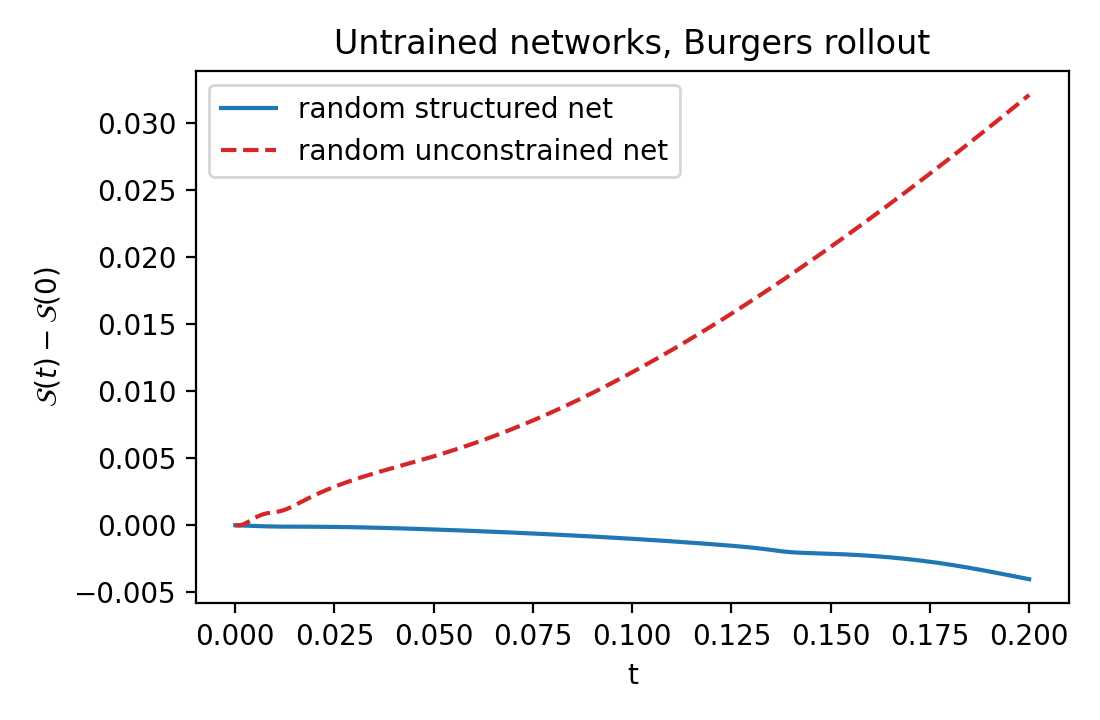
\includegraphics[width=0.55\textwidth]{figs/random_rollout_entropy.png}
\caption{Entropy along rollouts of \emph{untrained} networks (Burgers, $K=100$, $r=6$).}\label{fig:random}
\end{figure}

\paragraph{Observation for training (not a test failure).} In the smoke run, the first-epoch losses were:
\begin{center}\small
\begin{tabular}{lccc}
\toprule
network & data & teacher & entropy\\\midrule
structured & 1.24 & 1.14 & $2.4\times10^{2}$\\
unconstrained & 1.13 & 1.05 & $9.5\times10^{5}$\\
\bottomrule
\end{tabular}
\end{center}
The entropy loss is normalized by $\mathrm{mean}\,D_k^2$, which is small. A random network's dissipation is far from it, so even with weight 0.1 this term dominates the total loss once pretraining ends (epoch 3: total $20.6$, of which $18.7$ is the entropy term). For the unconstrained net this is expected, because its $v_N^T\dot a$ also contains the large reversible part. For the full runs, check \code{loss.png}: if the entropy term still dominates after pretraining, \code{w\_entropy} may need to be lowered, or its normalization changed.

%======================================================================
\section{Results: Burgers with the learned eddy-viscosity closure}\label{sec:results}
%======================================================================
\paragraph{Why the closure model.} Networks that learn the full reduced dynamics did not reach the ES-ROM's accuracy on Burgers with $r=16$. The best version (per-mode scaling $D$) had 17\% error at $T_{\rm train}$, against $10^{-6}$ for the ES-ROM. The ES-ROM computes the convective and viscous terms, which cancel to within 1/20--1/70 for modes $\ge5$, exactly; a generic matrix output cannot. The closure model \eqref{eq:closure} keeps those terms exact.

\paragraph{Setup.}
\begin{itemize}
\item \textbf{FOM:} Burgers with $u_0=-\sin\pi x$, $K=1000$, $\epsilon=2\times10^{-3}$ and $\Delta t=5\times10^{-4}$.
\item \textbf{Data:} basis and training data from $t\le0.75$; rollouts to $T=1.5$ with the FOM time step.
\item \textbf{Number of modes:} with $r=16$ the ES-ROM is essentially exact, so there is nothing to close. The closure was therefore tested at $r=4$ and $r=6$, where the ES-ROM error is well above the projection error (Table~\ref{tab:rscan}).
\item \textbf{Training:} 30\,000 epochs, Adam, CPU. Each run took about 8\,min (12--20\,ms per epoch); the MLP outputs only $r$ numbers.
\item \textbf{Reported:} final weights.
\end{itemize}

\begin{table}[h]\centering
\caption{Relative $L^2$ error against the FOM for different basis sizes. Projection: the best error possible in $\mathrm{span}(V)$.}\label{tab:rscan}
\begin{tabular}{ccccc}
\toprule
$r$ & projection, $t=0.75$ & ES-ROM, $t=0.75$ & projection, $t=1.5$ & ES-ROM, $t=1.5$\\\midrule
3 & $3.3\times10^{-2}$ & $8.7\times10^{-2}$ & $3.3\times10^{-2}$ & $7.4\times10^{-2}$\\
4 & $3.2\times10^{-3}$ & $3.4\times10^{-2}$ & $2.5\times10^{-2}$ & $1.7\times10^{-1}$\\
5 & $2.3\times10^{-3}$ & $1.1\times10^{-2}$ & $2.1\times10^{-2}$ & $1.4\times10^{-1}$\\
6 & $1.8\times10^{-3}$ & $6.3\times10^{-3}$ & $1.1\times10^{-2}$ & $7.4\times10^{-2}$\\
8 & $4.5\times10^{-4}$ & $1.9\times10^{-3}$ & $1.0\times10^{-3}$ & $6.6\times10^{-3}$\\
16 & $1.8\times10^{-7}$ & $1.2\times10^{-6}$ & $3.8\times10^{-7}$ & $6.0\times10^{-6}$\\
\bottomrule
\end{tabular}
\end{table}

\begin{table}[h]\centering
\caption{ES-ROM + learned viscosity against Chan's ES-ROM (relative $L^2$ error against the FOM; $t=0.75$ is the end of the training window). POD--Galerkin is identical to the ES-ROM for Burgers ($v=u$). ``At start'': the ES-ROM's data loss before training.}\label{tab:closure}
\begin{tabular}{lcccc}
\toprule
& \multicolumn{2}{c}{$r=4$} & \multicolumn{2}{c}{$r=6$}\\
& $t=0.75$ & $t=1.5$ & $t=0.75$ & $t=1.5$\\\midrule
projection (lower bound) & $3.2\times10^{-3}$ & $2.5\times10^{-2}$ & $1.8\times10^{-3}$ & $1.1\times10^{-2}$\\
ES-ROM (Chan) & $3.37\times10^{-2}$ & $1.67\times10^{-1}$ & $6.27\times10^{-3}$ & $7.40\times10^{-2}$\\
\textbf{ES-ROM + learned viscosity} & $\mathbf{7.40\times10^{-3}}$ & $2.03\times10^{-1}$ & $\mathbf{5.47\times10^{-3}}$ & $\mathbf{3.31\times10^{-2}}$\\
improvement over ES-ROM & $4.6\times$ & $0.82\times$ (worse) & $1.15\times$ & $2.2\times$\\\midrule
final data loss (at start) & \multicolumn{2}{c}{$1.0\times10^{-2}$ ($6.4\times10^{-2}$)} & \multicolumn{2}{c}{$6.1\times10^{-4}$ ($3.9\times10^{-2}$)}\\
mean / max $\nu_\theta/\epsilon$ along rollout & \multicolumn{2}{c}{0.96 / 105} & \multicolumn{2}{c}{0.30 / 23}\\
\bottomrule
\end{tabular}
\end{table}

\begin{figure}[h]\centering
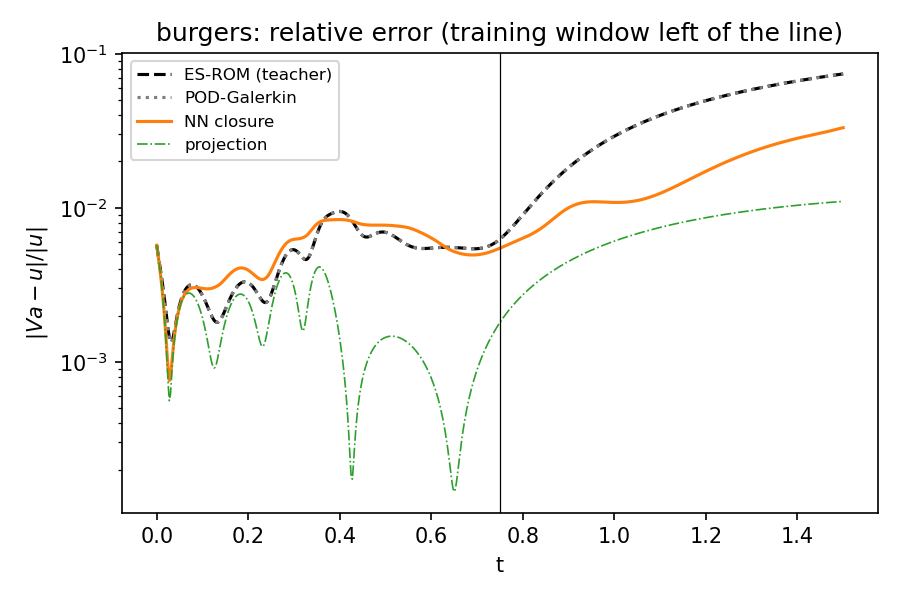
\includegraphics[width=0.49\textwidth]{figs/closure_r6_error.png}\hfill
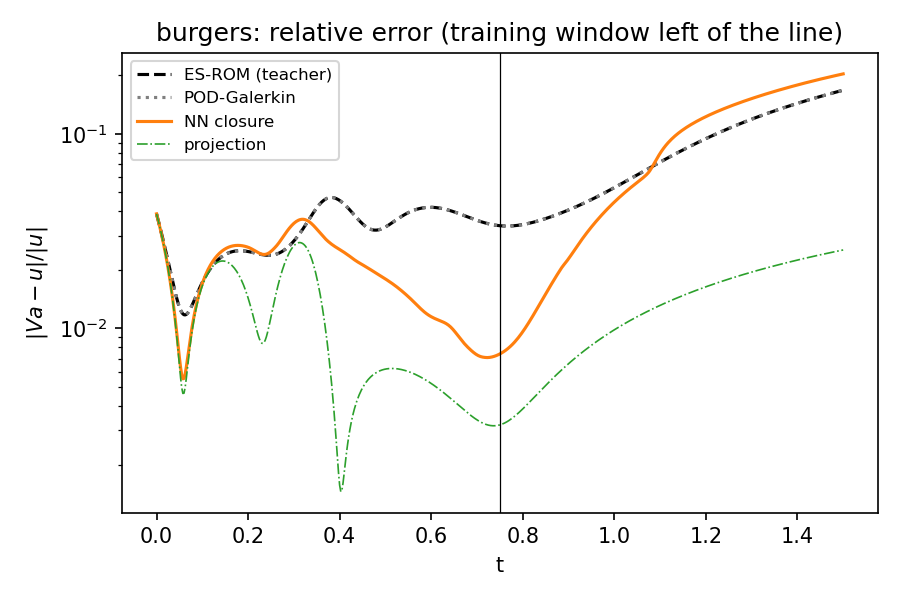
\includegraphics[width=0.49\textwidth]{figs/closure_r4_error.png}
\caption{Error against the FOM over time. Left: $r=6$. Right: $r=4$. The vertical line is the end of the training window.}\label{fig:closure-err}
\end{figure}

\begin{figure}[h]\centering
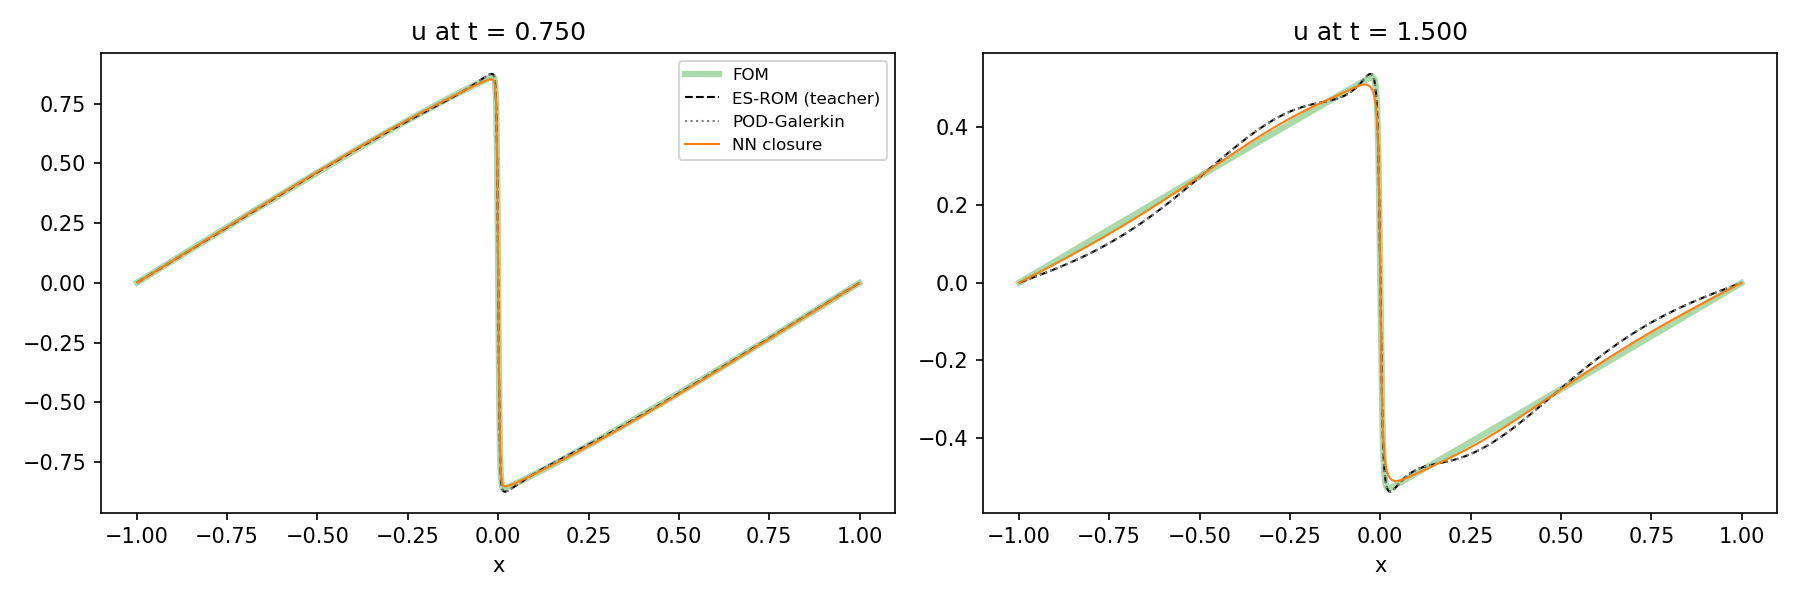
\includegraphics[width=\textwidth]{figs/closure_r6_profiles.png}
\caption{$r=6$: solution at the end of training ($t=0.75$) and at the end of the rollout ($t=1.5$). At $t=1.5$ the ES-ROM shows truncation wiggles away from the shock; the closure removes most of them.}\label{fig:closure-prof}
\end{figure}

\begin{figure}[h]\centering
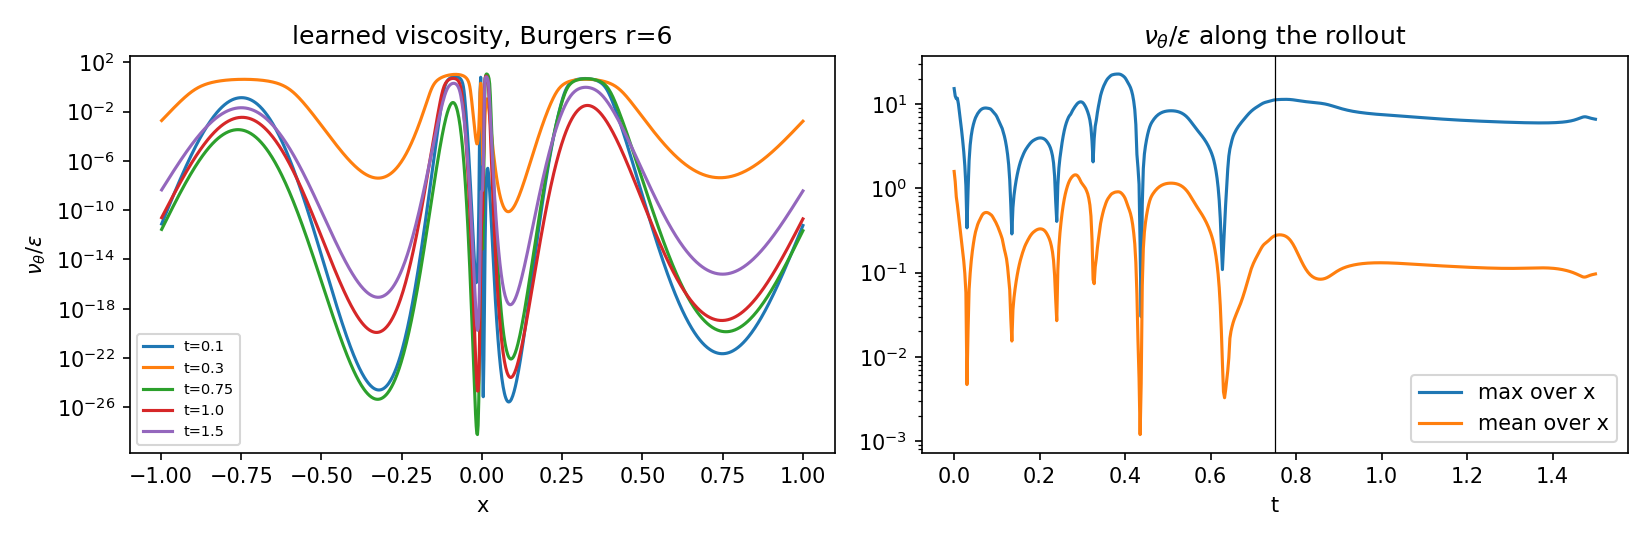
\includegraphics[width=\textwidth]{figs/closure_r6_viscosity.png}\\[2pt]
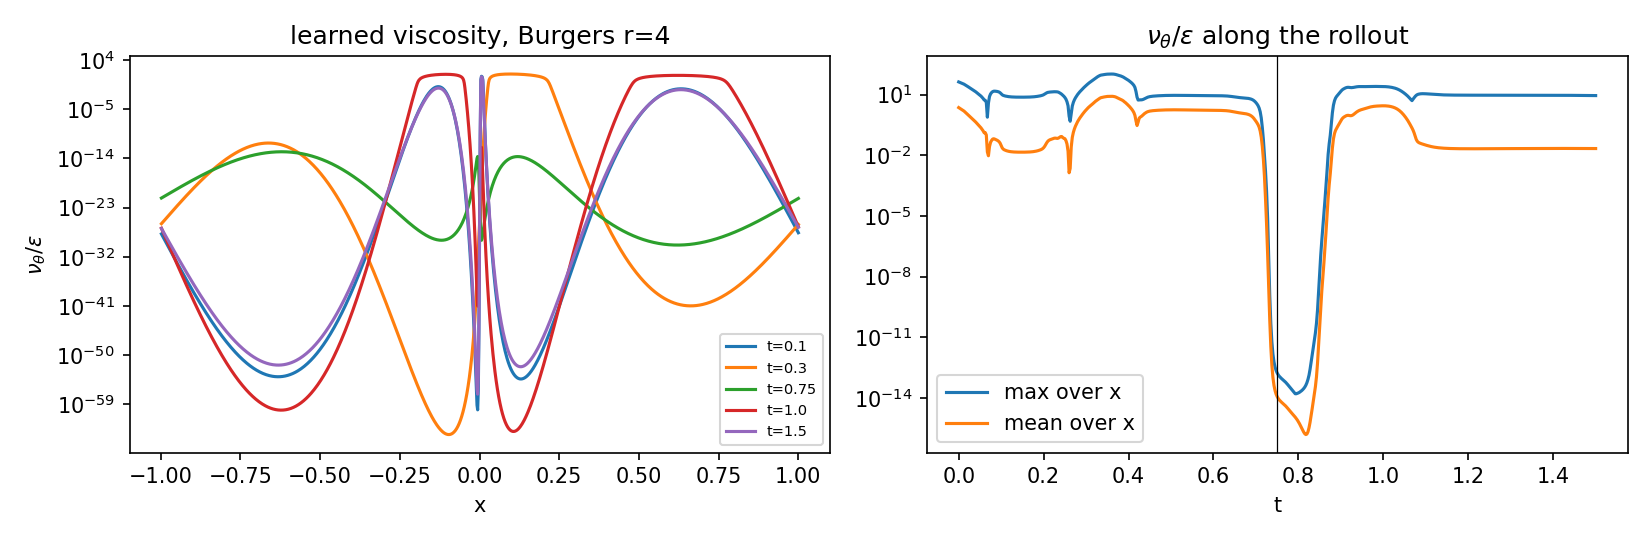
\includegraphics[width=\textwidth]{figs/closure_r4_viscosity.png}
\caption{Learned viscosity $\nu_\theta/\epsilon$. Left: in space at five times (log scale). Right: maximum and mean over $x$ along the rollout. Top: $r=6$. Bottom: $r=4$.}\label{fig:closure-nu}
\end{figure}

\needspace{8\baselineskip}\paragraph{Findings.}
\begin{enumerate}
\item \textbf{The closure beats Chan's ES-ROM, and the guarantees hold.} For $r=6$ the end-time error halves ($7.4\%\to3.3\%$), and the gain \emph{grows} in the extrapolation window (Fig.~\ref{fig:closure-err}, left; Fig.~\ref{fig:closure-prof}). Along both trained trajectories:
  \begin{itemize}
  \item the closure's entropy rate is $\le0$ everywhere (max $-1.2\times10^{-4}$ for $r=6$, $-1.7\times10^{-16}$ for $r=4$);
  \item $\Sc(t)$ never increases;
  \item the totals are conserved to round-off.
  \end{itemize}
\item \textbf{The viscosity is localized.} It concentrates near the shock (up to about $10$--$20\,\epsilon$ for $r=6$) and is essentially zero in large parts of the domain (Fig.~\ref{fig:closure-nu}, top). This matches what a VMS / eddy-viscosity closure should do.
\item \textbf{For $r=4$ the gain is limited to the training window.} Inside it the error drops $4.6\times$. Right after $t=0.75$ the learned viscosity switches off completely (its maximum falls to about $10^{-14}\epsilon$ for $t\approx0.75$--$0.85$), and the end error is worse than the ES-ROM's (Fig.~\ref{fig:closure-err}, right; Fig.~\ref{fig:closure-nu}, bottom).
\item \textbf{Weakness of the parameterization.} The learned field spans $10^{-130}$--$10^{2}\epsilon$, because $z$ uses very large coefficients inside the softplus. The viscosity can therefore jump between ``off'' and ``on'' at almost no cost in the loss, which explains the $r=4$ behaviour. Bounding $z$, or building $\nu$ as a positive combination of the $\phi_k$, should give a smoother field that is easier to extrapolate.
\item \textbf{A viscosity cannot close everything.} For $r=4$ the data loss levels off at $1.0\times10^{-2}$. Part of the truncation error there is not dissipative, and a viscosity can only add dissipation.
\end{enumerate}
Output folders: \code{outputs/burgers\_r4/} and \code{outputs/burgers\_r6/} (figures, \code{metrics.json}, logs).

%======================================================================
\section{Status and next step}
%======================================================================
\begin{itemize}
\item All 33 unit tests pass (29 + 4 closure tests). The physics, FOM, basis, teacher, network structure and closure behave as designed, with the invariants at round-off ($10^{-14}$--$10^{-17}$).
\item One test reference was corrected (Sec.~\ref{sec:t-physics}). After the first Burgers training, the scalar output scale $s$ was replaced by the per-mode scaling $D$ (Sec.~\ref{sec:arch}); \code{test\_model.py} was rerun with $D$ (7/7 pass), and the network numbers in Sec.~\ref{sec:t-model} are from that version.
\item Files added for this report: \code{tests/run\_tests.py} (runner) and \code{report/} (this document, \code{measure\_invariants.py}, figures, logs).
\item Burgers results (Sec.~\ref{sec:results}): the ES-ROM + learned viscosity closure beats Chan's ES-ROM. The gain is $2.2\times$ at the end time for $r=6$, and $4.6\times$ inside the training window for $r=4$. Extrapolation at $r=4$ fails because the viscosity switches off.
\item \textbf{Open} (on request):
  \begin{itemize}
  \item a smoother viscosity parameterization (bounded $z$, or a positive combination);
  \item a closure that is not only dissipative, for small $r$;
  \item the Euler pulse.
  \end{itemize}
\end{itemize}

\end{document}
